\section{BlkKin Evaluation}

\begin{frame}[t]{Outline}
\setcounter{tocdepth}{1}
\tableofcontents[currentsection]
\end{frame}

\subsection{Overview}
\begin{frame}{Evaluation Environment}
Instrumented:
\begin{itemize}
\item QEMU Archipelago driver
\item Archipelago and libxseg
\item RADOS
\end{itemize}
\hfill \\
\hfill \\
Testbed:
\begin{itemize}
\item 2 hosts interconnected over LAN
\item 2 OSDs per host
\item 1 host running QEMU and Archipelago
\end{itemize}
\end{frame}

\begin{frame}{Zipkin in Action}
\hfill \\
\begin{center}
{\Large Zipkin Demo}
\end{center}
\end{frame}

\subsection{Metrics}
\begin{frame}{I/O Loads - Scenarios}
I/O loads created within VM using \texttt{fio}:
\begin{itemize}
\item 4k random writes
\item 64k sequential writes
\end{itemize}
\hfill \\
\hfill \\
Scenarios:
\begin{itemize}
\item no tracing
\item stopped tracing
\item normal tracing
\item live tracing without sampling
\item live tracing with 1/500 sampling
\end{itemize}
\end{frame}

\begin{frame}[t]{Bandwidth Overhead}
\begin{center}
\begin{columns}
    \begin{column}{0.5\textwidth}
        \begin{center}
            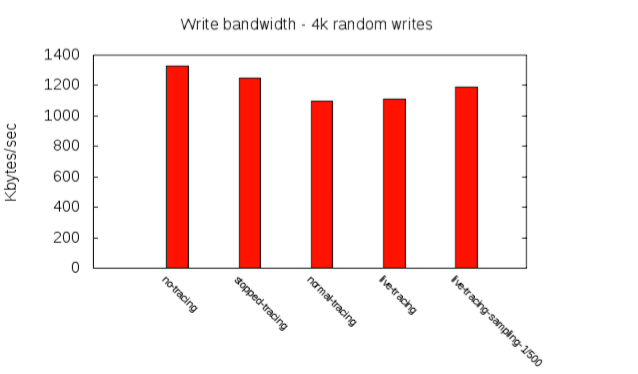
\includegraphics[scale=0.3]{images/4.png}
        \end{center}
    \end{column}
    \begin{column}{0.5\textwidth}
        \begin{center}
            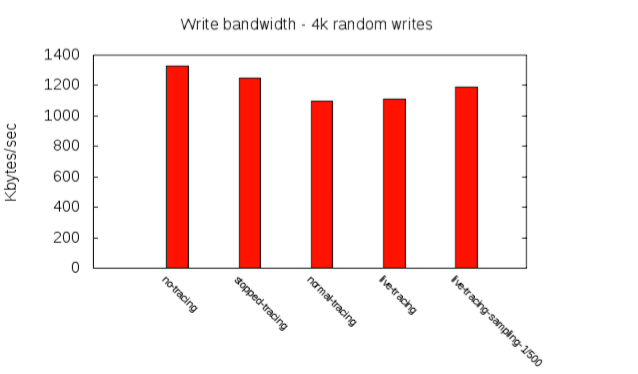
\includegraphics[scale=0.3]{images/4.png}
        \end{center}
    \end{column}
\end{columns}
\end{center}
\end{frame}

\subsection{Detecting Problems}

\begin{frame}{Fault injection}
\begin{enumerate}
\item Calculate threshold values using MapReduce in HDFS
\hfill \\
\hfill \\
\item Simulate faulty environment:
    \begin{itemize}
    \item Network faults: using \texttt{tc}
    \item Disk faults: adding extra I/O load using \texttt{fio}
    \end{itemize}
\hfill \\
\hfill \\
\item Detect faults using BlkKin monitoring UI
\end{enumerate}
\end{frame}

\begin{frame}{Network fault}
 \makebox[\textwidth][c]{
        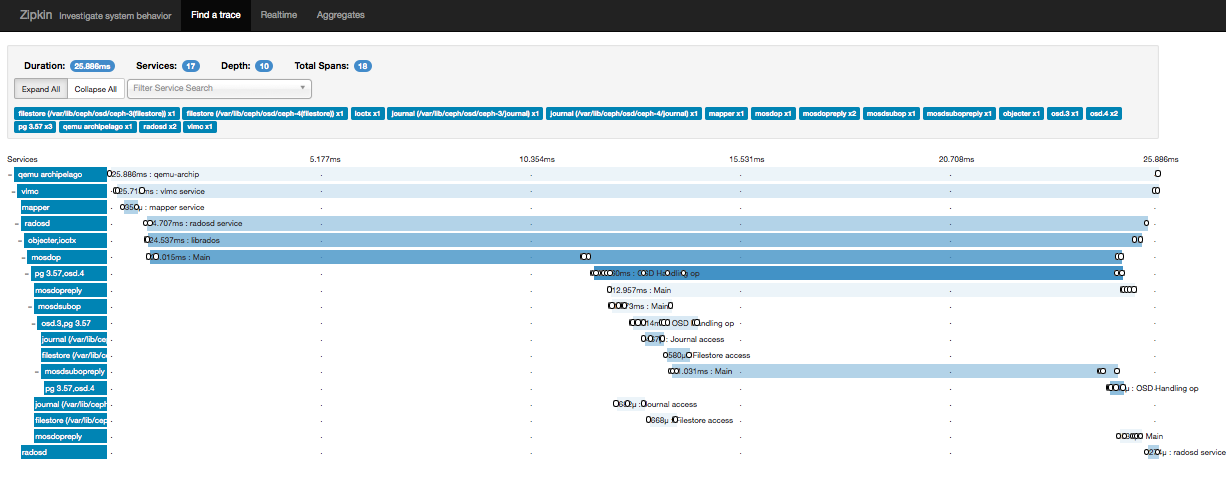
\includegraphics[width=\paperwidth,
height=0.6\paperheight]{images/network-error.png}
}
\end{frame}

\begin{frame}{Network fault}
\begin{center}
% \makebox[\textwidth][c]{
%        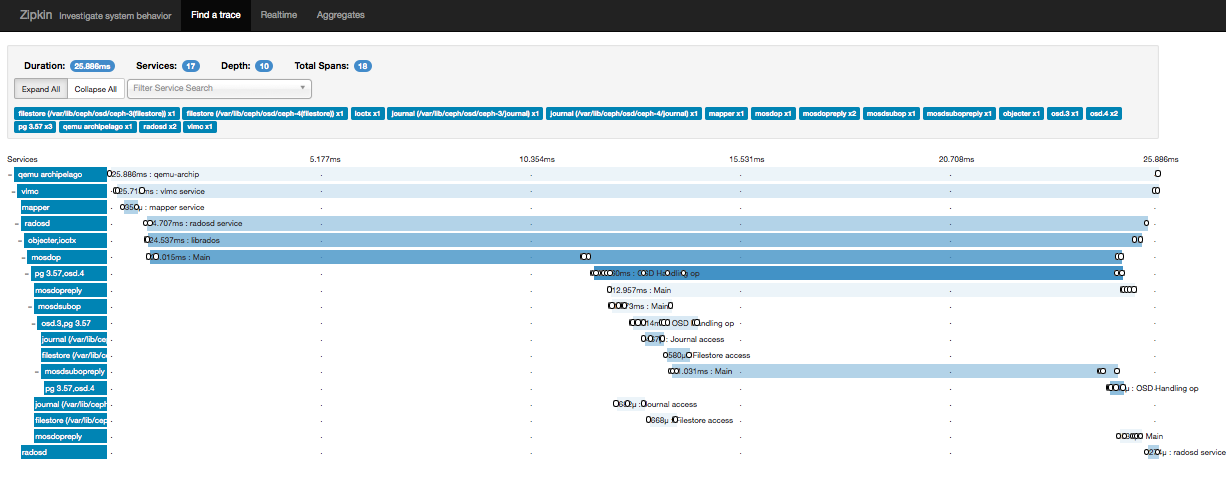
\includegraphics[width=\paperwidth,
%height=0.5\paperheight]{images/network-error.png}
%}
 \makebox[\textwidth][c]{
        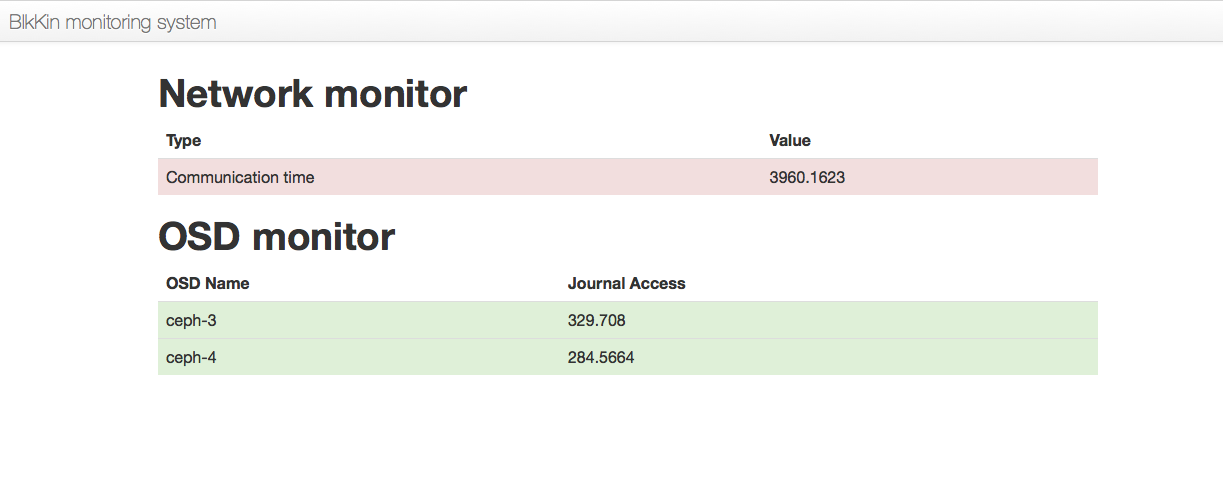
\includegraphics[width=\paperwidth, keepaspectratio=true]{images/network-error-blkin.png}
}
\end{center}
\end{frame}


\begin{frame}{Disk fault}
\begin{center}
% \makebox[\textwidth][c]{
%        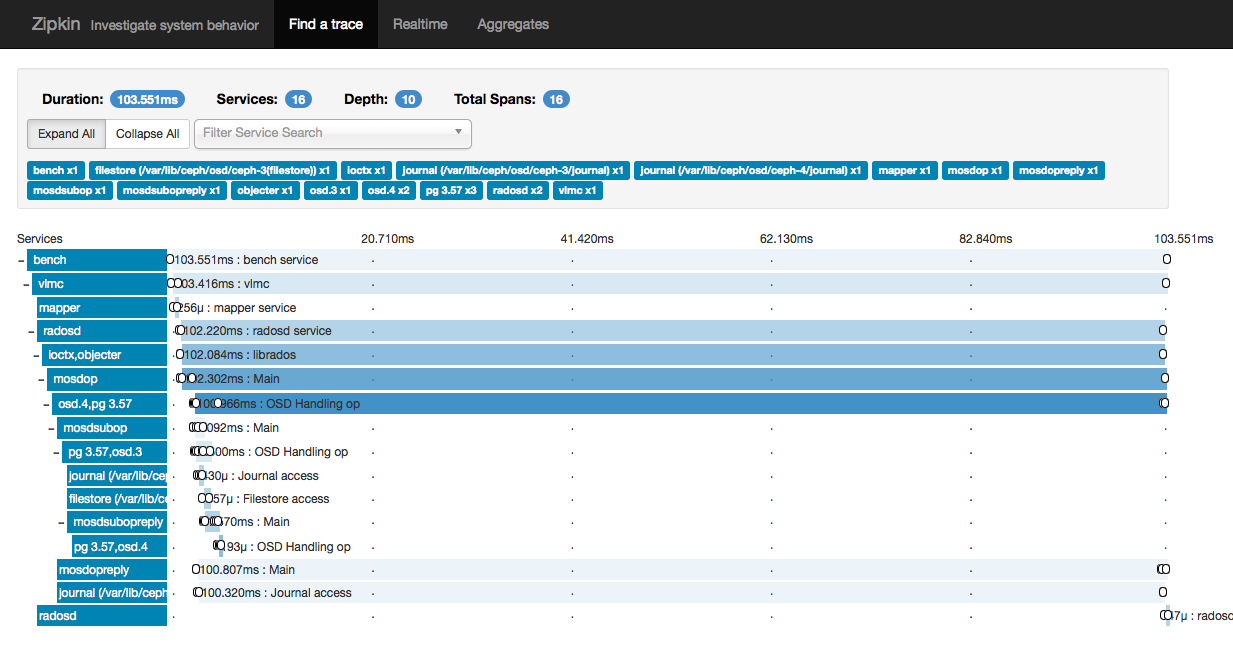
\includegraphics[width=\paperwidth,
%height=0.5\paperheight]{images/disk-fault.png}
%}
 \makebox[\textwidth][c]{
        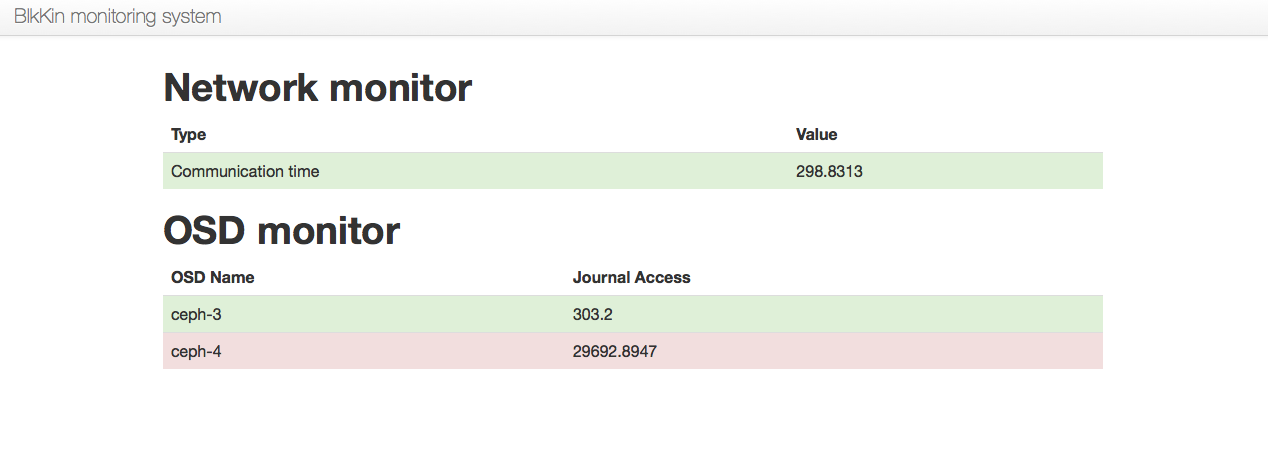
\includegraphics[width=\paperwidth,keepaspectratio=true]{images/disk-fault-blkin.png}
}
\end{center}
\end{frame}
